\subsubsection{Di-Higgs production in the non-linear EFT with full $m_t$-dependence at NLO QCD}

\begin{center}
\textit{by Gerhard Buchalla, Alejandro Celis, Matteo Capozi, Gudrun Heinrich, Ludovic Scyboz}
\end{center}


\subsubsubsection{The Higgs sector in the non-linear EFT framework}
\label{sec:EWChL.double.h}

Below we will describe  the potential impact of physics
beyond the Standard Model through a non-linear Effective Field Theory,
also called the electroweak chiral Lagrangian
including a light Higgs 
boson~\cite{Buchalla:2013rka,Buchalla:2013eza,Buchalla:2017jlu}.
This framework provides us with a consistent EFT
for New Physics in the Higgs sector, where the Higgs field is an electroweak singlet $h$,
independent of the Goldstone matrix $U = \exp(2i\varphi^a T^a/v)$.
The latter transforms as $U\to g_L U g^\dagger_Y$ under the SM gauge group.
The symmetry is non-linearly realised on the Goldstone fields
$\varphi^a$, therefore the name non-linear EFT.
More details about this framework already have been given in
Section~\ref{sec:2:kappavsEFT}.
Therefore we restrict ourselves to stating the part of the Lagrangian
relevant for our study of anomalous Higgs couplings:
\begin{align}
{\cal L}\supset 
-m_t\left(c_t\frac{h}{v}+c_{tt}\frac{h^2}{v^2}\right)\,\bar{t}\,t -
c_{hhh} \frac{m_h^2}{2v} h^3+\frac{\alpha_s}{8\pi} \left( c_{ggh} \frac{h}{v}+
c_{gghh}\frac{h^2}{v^2}  \right)\, G^a_{\mu \nu} G^{a,\mu \nu}\;.
\label{eq:ewchl}
\end{align}
To lowest order in the SM $c_t=c_{hhh}=1$ and $c_{tt}=c_{ggh}=c_{gghh}=0$.
In general, all couplings may have arbitrary values of ${\cal O}(1)$.
Note that we have extracted a loop factor from the definition of the
Higgs-gluon couplings.  


The leading-order diagrams are shown in Fig.~\ref{fig:hprocess}.
\begin{figure}[htb]
\begin{center}
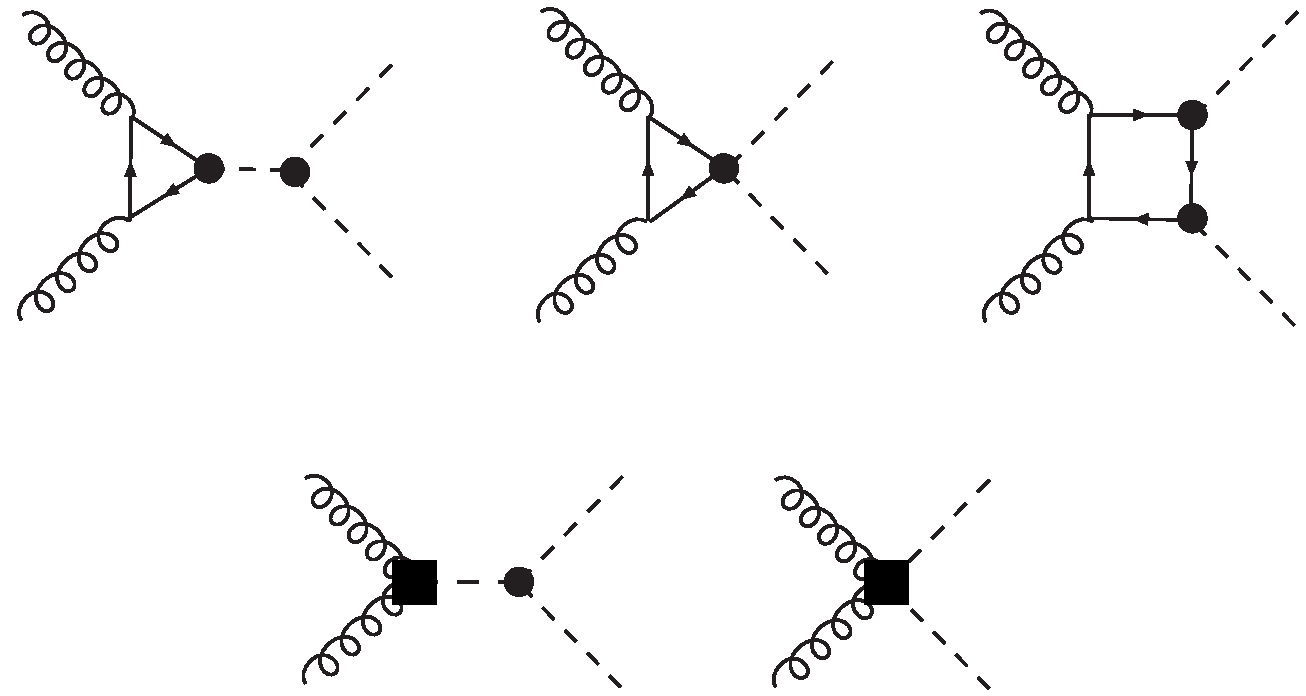
\includegraphics[width=7.5cm]{\main/section3/plots/hprocess.pdf}
\end{center}
\caption{Higgs-pair production in gluon fusion at leading order
in the non-linear EFT Lagrangian.}
\label{fig:hprocess}
\end{figure}
Examples for virtual diagrams at NLO are shown in
Fig.~\ref{fig:virt_examples}.
For further details we refer to Ref.~\cite{Buchalla:2018yce}.
\begin{figure}[htb]
\begin{center}
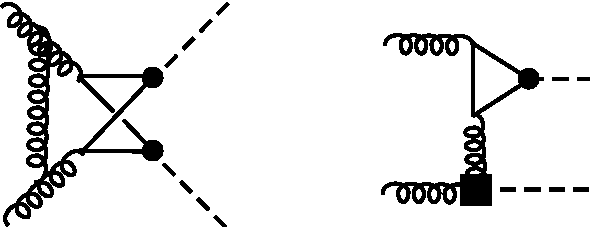
\includegraphics[width=6cm]{\main/section3/plots/hpnloyr1.pdf}
\end{center}
\caption{Examples of virtual diagrams contributing at NLO QCD.}
\label{fig:virt_examples}
\end{figure}


\subsubsubsection{Total cross sections for 14 and 27 TeV at some benchmark points}

In the following we will show results for some benchmark points, specified in Table~\ref{tab:benchmarks}, 
some of them having been first defined in Refs.~\cite{Carvalho:2015ttv}.
The results at 14\,TeV and 27\,TeV are given in Table~\ref{sigmatot}.
Note that our conventions for $\cg$ and $\cgg$ differ from the ones in
Ref.~\cite{Carvalho:2015ttv,Carvalho:2016rys}, the relations are $c_{ggh}= \frac{2}{3}c_g $
and $c_{gghh}=-\frac{1}{3}c_{2g}$, where $c_g,c_{2g}$ are the
couplings defined in Refs.~\cite{Carvalho:2015ttv,Carvalho:2016rys}.
We also take into account recent constraints on $\cg$ from
Refs.~\cite{CMS-PAS-HIG-17-031,deBlas:2018tjm}
and the  limits on the Higgs boson pair production cross section
from Refs~\cite{CMS-PAS-HIG-17-030,ATLAS-CONF-2018-043}.
This is why we do not show results for the original benchmark point 5
anymore, as its value for $\cg$ is outside the 2-sigma band of a
combined fit of $\cg,\ct$ from single Higgs production
data~\cite{CMS-PAS-HIG-17-031,deBlas:2018tjm}.
Benchmark point 6 is interesting because its value for $\chhh$ is near
the point where maximal destructive interference takes place between
triangle-type and box-type contributions if the other couplings are SM-like, leading to a total cross
section which is below the SM value.

\begin{table}[htb]
\begin{center}
%\setlength{\extrarowheight}{3.0pt}
%\scalebox{1.}{%
\begin{tabular}{| c | c  c  c  c  c |}
%\Xhline{2\arrayrulewidth}
\hline
Benchmark & $c_{hhh}$ & $c_t$ & $c_{tt}$ & $c_{ggh}$ & $c_{gghh}$ \\
\hline
5a & 1 & 1 & 0 &   $2/15$ & $4/15$\\
\hline
6 & 2.4 & 1 & 0 & $2/15$ & $1/15$  \\
\hline
7 & 5 & 1 & 0 & $2/15$ & $1/15$  \\
\hline
8a & 1 & 1 & 1/2 & $4/15$ & 0\\
\hline
SM & 1 & 1 & 0 & 0 & 0 \\
\hline
%\Xhline{2\arrayrulewidth}
\end{tabular}
\end{center}
\caption{Benchmark points used for the distributions shown below.\label{tab:benchmarks}}
\end{table}
%
\begin{table}[htb]
\begin{center}
\begin{tabular}{|c|c|c|c|c|c|}
\hline
&&&&&\\
Benchmark & $\sigma_{NLO}$ [fb] & K-factor & scale uncert.  &
stat. uncert.   &$\frac{\sigma_{NLO}}{\sigma_{NLO,SM}}$ \\ 
&&&[\%] &[\%] &\\
\hline
$    B_{5a}$ [14 TeV] & 38.64 & 1.78& ${+3.7, \; -12}$ &0.24  &1.17  \\ 
$    B_{5a}$ [27 TeV] & 198.64 & 1.75 & ${+2.1, \; -10}$ & 0.43 & 1.56  \\ 
\hline
$    B_{6}$ [14 TeV] &  24.69 & 1.89 & ${+2, \; -11}$ & 2.1 & 0.75 \\ 
$    B_{6}$ [27 TeV] &  97.25 &  1.58& ${+0.53, \; -5.6}$ &1.63  & 0.76  \\ 
\hline
$   B_7$ [14 TeV] & 169.41 & 2.07& ${+9, \; -12}$ & 2.2 & 5.14 \\
$   B_7$ [27 TeV] & 598.20 & 2.11 & ${+8, \; -10}$ & 2.0 &  4.68\\
\hline 
$   B_{8a}$ [14 TeV] & 41.70 & 2.34& ${+6, \; -9}$ & 0.63 & 1.27 \\
$   B_{8a}$ [27 TeV] & 179.52 & 2.33 & ${+4, \; -7}$ & 0.49 & 1.40 \\
\hline 
$   SM $ [14 TeV] & 32.95 & 1.66 & ${+14, \; -13}$ & 0.1 & 1\\
$   SM $ [27 TeV] & 127.7&  1.62 & ${+12, \; -10}$ & 0.1 & 1\\
\hline
\end{tabular}
\end{center}
\caption{Total cross sections at 14 and 27 TeV at NLO (2nd column),
K-factor $\sigma_{NLO}/\sigma_{LO}$ (3rd column),
scale uncertainty (4th column), statistical uncertainty (5th column)
and the ratio to the SM total cross section at NLO (6th column).\label{sigmatot}}
\end{table}
%
% \begin{table}[htb]
% \begin{center}
% \begin{tabular}{|c|c|c|c|c|}
% \hline
%  & $B_5$ & $B_7$ & $B_{8a}$& SM\\
% \hline
% $\frac{\sigma_{NLO}[27\,\mathrm{TeV}]}{\sigma_{NLO}[14\,\mathrm{TeV}]}$& 5.10& 3.53& 4.31& 3.88\\
% \hline
% \end{tabular}
% \end{center}
% \caption{Ratios of total cross sections at 14\,TeV and 27\,TeV at NLO.\label{energy_ratios}}
% \end{table}
Table~\ref{sigmatot} shows that the total cross sections increase by a factor of 3.5-5 when increasing the centre-of-mass energy from 14\,TeV to 27\,TeV. The increase for $B_{5a}$ is largest because of the large value of $\cgg$, which yields a contribution growing linearly with energy.

%\clearpage


\subsubsubsection{HH  invariant mass distributions at 14 and 27 TeV at some benchmark points}

In Figs.~\ref{fig:benchmark7} and \ref{fig:benchmark8a} we show Higgs boson pair invariant mass distributions for the benchmark points 7 and 8a. 
For both of them the shape of the distribution is very different from the SM one, and the K-factor is non-homogeneous over the whole $\mhh$-range. Benchmark point 7 is characterised by a large enhancement of the low $\mhh$ region, induced by the large value of $\chhh$. The lower ratio plot shows the ratio of the two approximations ``Born-improved HEFT" and ``FT$_{\rm{approx}}$" to the full NLO, where the former denotes the $m_t\to\infty$ limit rescaled by the $m_t$-dependent LO, while FT$_{\rm{approx}}$ includes the Born-improved $m_t\to\infty$ limit for the virtual part and the full $m_t$-dependence for the real radiation part. One can see from Fig.~\ref{fig:benchmark7} that these approximations are off by about 20\% even below the $2m_t$ threshold. Therefore one cannot claim that the $m_t\to \infty$ limit works well in the region below $\sim 400$\,GeV. As the triangle-type contributions are dominating for $\chhh=5$, their full $m_t$-dependence plays a significant role. 

Benchmark point 8a shows a characteristic dip near $\mhh=2\,m_t$ and an enhancement in the tail compared to the SM. 
As the total cross section for $B_{8a}$ is very similar to the SM one, both at 14\,TeV and at 27\,TeV, this is an example where the discriminating power of differential information is very important.

\begin{figure}[htb]
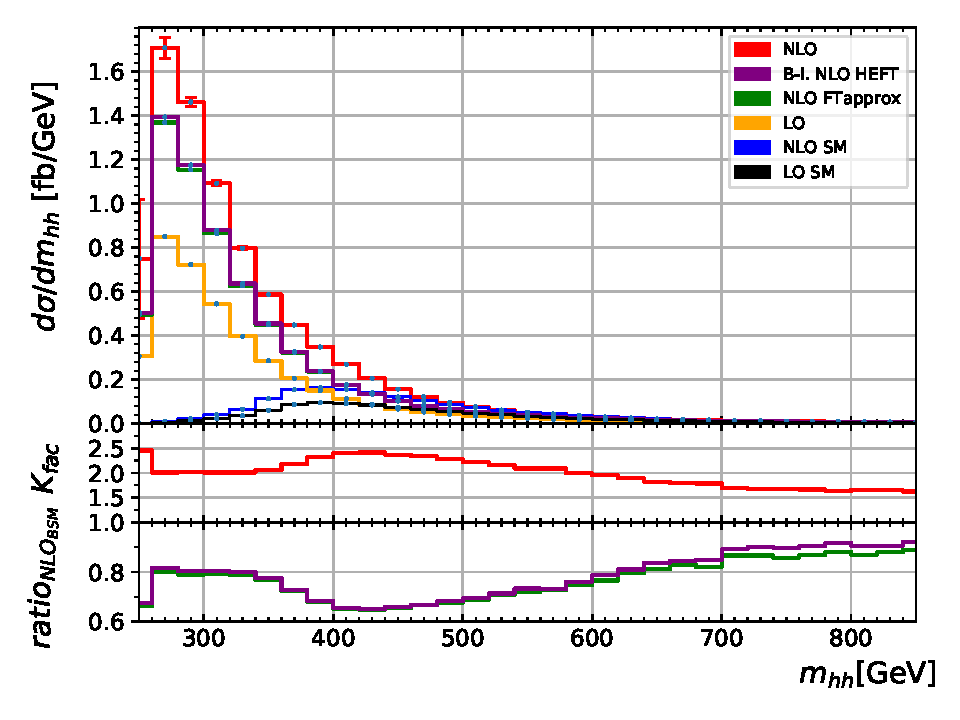
\includegraphics[width=0.48\textwidth]{\main/section3/plots/Ben_7_mhh.pdf}
~
 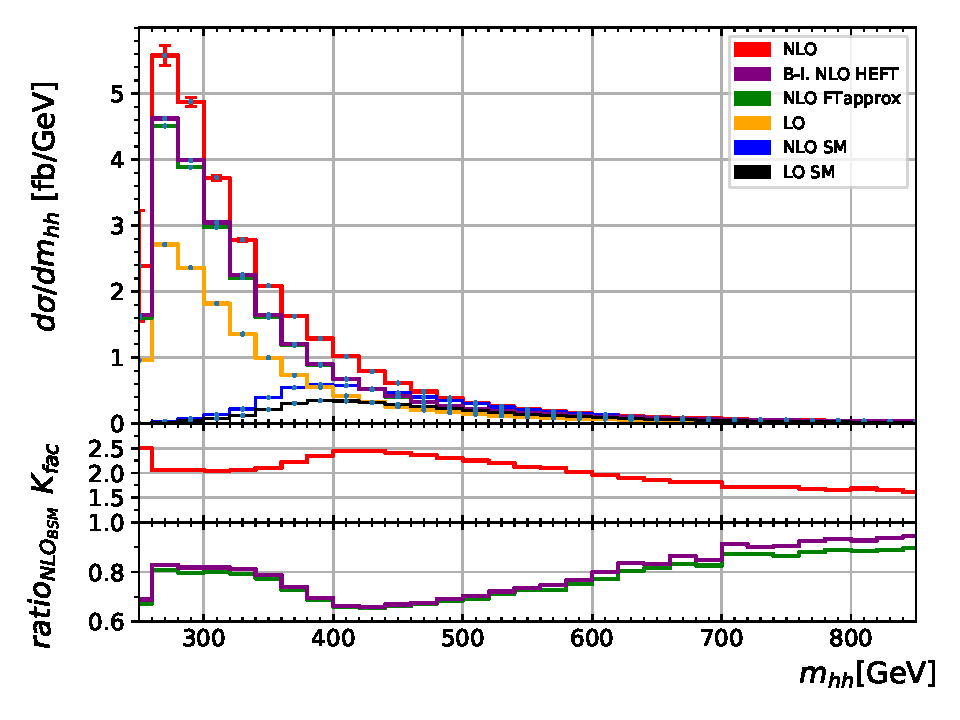
\includegraphics[width=0.48\textwidth]{\main/section3/plots/Ben_7_mhh_27TeV.pdf}
\caption{Higgs boson pair invariant mass distributions  for benchmark point 7, $\chhh=5,\ct= 1, \ctt=0, \cg=2/15,\cgg=1/15$, at 14\,TeV (left) and 27\,TeV (right).}
\label{fig:benchmark7}
\end{figure}
%
\begin{figure}[htb]
  \centering
  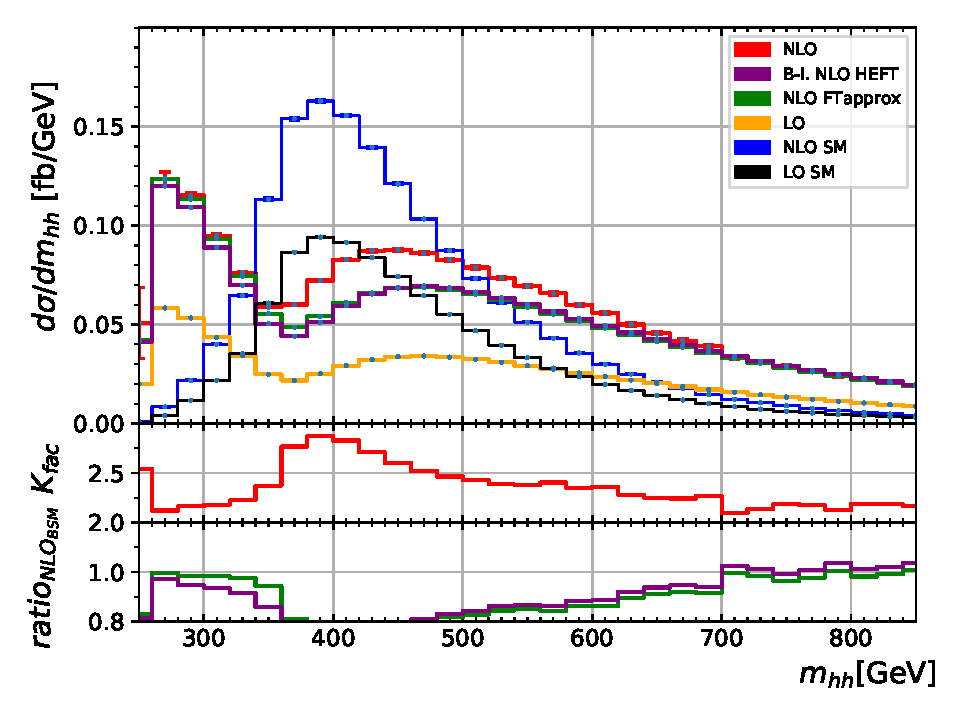
\includegraphics[width=0.48\textwidth]{\main/section3/plots/Ben_8a_mhh.pdf} 
~
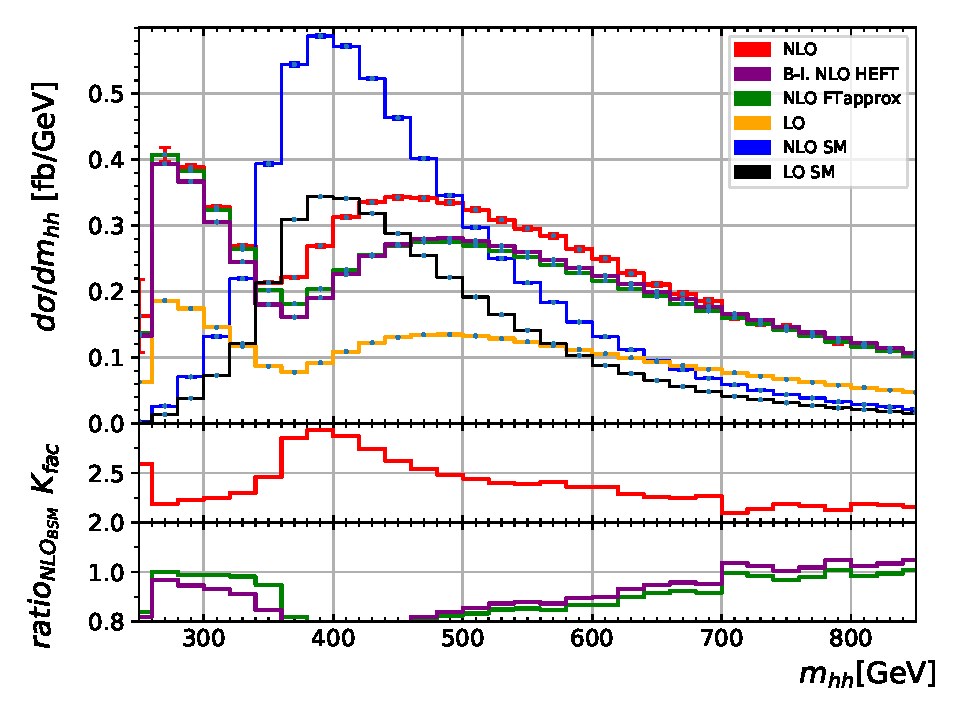
\includegraphics[width=0.48\textwidth]{\main/section3/plots/Ben_8a_mhh_27TeV.pdf}
\caption{Higgs boson pair invariant mass distributions  for benchmark point 8a, $\chhh=1,\ct= 1, \ctt=0.5, \cg=4/15,\cgg=0$, at 14\,TeV (left) and 27\,TeV (right).}
\label{fig:benchmark8a}
\end{figure}
%



\subsubsubsection{Characterising the BSM parameter space}

The total cross section can be written in terms of the 15 coefficients 
$A_1, \ldots, A_{15}$, at LO~\cite{Carvalho:2015ttv,Azatov:2015oxa} and in terms of 23 coefficients at NLO~\cite{Buchalla:2018yce}.
%
\begin{align}
\label{eq:Acoeffs_all}
&\sigma^{\rm{NLO}}/\sigma^{\rm{NLO}}_{SM}  =\nn\\
& \quad  A_1\, c_t^4 + A_2 \, c_{tt}^2  + A_3\,  c_t^2 \chhh^2  + 
A_4 \, \cg^2 \chhh^2  + A_5\,  \cgg^2  + 
A_6\, c_{tt} c_t^2 + A_7\,  c_t^3 \chhh \nn\\
& + A_8\,  c_{tt} c_t\, \chhh  + A_9\, c_{tt} \cg \chhh + A_{10}\, c_{tt} \cgg + 
A_{11}\,  c_t^2 \cg \chhh + A_{12}\, c_t^2 \cgg \nn\\
& + A_{13}\, c_t \chhh^2 \cg  + A_{14}\, c_t \chhh \cgg +
A_{15}\, \cg \chhh \cgg \nn\\ 
& + A_{16}\, c^3_t \cg + A_{17}\,  c_t c_{tt} \cg 
+ A_{18}\, c_t \cg^2 \chhh + A_{19}\, c_t \cg \cgg 
\nn\\
&+ A_{20}\,  c_t^2 \cg^2 + A_{21}\, c_{tt} \cg^2 
+ A_{22}\, \cg^3 \chhh + A_{23}\, \cg^2 \cgg\,.
\end{align}
Based on our results for $A_1,\ldots, A_{23}$, we produce heat maps for the ratio $\sigma/\sigma_{SM}$, 
varying two of the five parameters, while for the fixed parameters the SM values are used, along with
$\sigma_{SM}^{\rm{LO}}[14\,\mathrm{TeV}]=19.85$\,fb,
$\sigma_{SM}^{\rm{NLO}}[14\,\mathrm{TeV}]=32.95$\,fb.
The couplings are varied in a range which seems reasonable when taking into account the current constraints on the 
Higgs coupling measurements
%~\cite{Khachatryan:2016vau}, 
as well as recent limits on the di-Higgs production cross
section~\cite{CMS-PAS-HIG-17-030,ATLAS-CONF-2018-043}.

%
\begin{figure}[ht]
\begin{center}
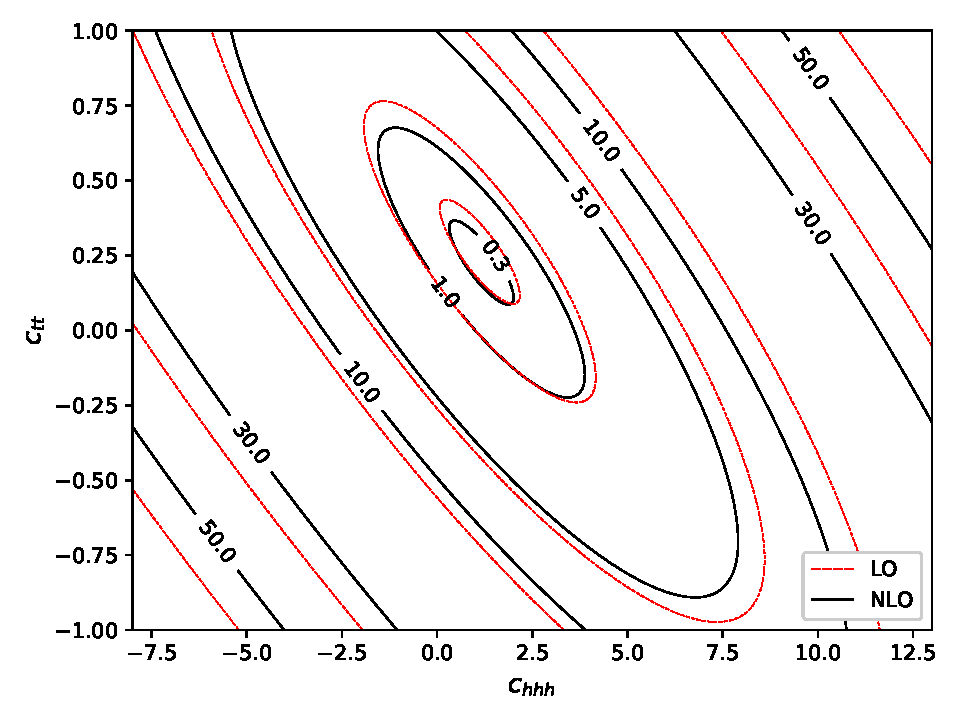
\includegraphics[width=0.45\textwidth]{\main/section3/plots/plot_chhh_ctt.pdf}    
~
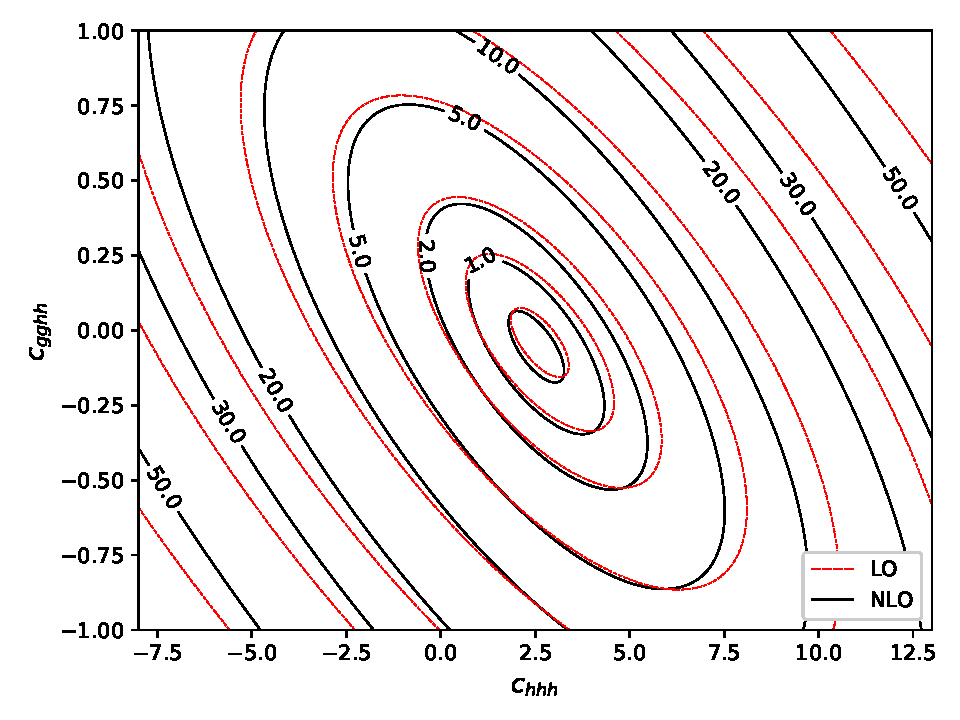
\includegraphics[width=0.45\textwidth]{\main/section3/plots/plot_chhh_cgghh.pdf}
\end{center}
\caption{Iso-contours of $\sigma/\sigma_{SM}$: (a) $\chhh$ versus $\ctt$ and (b) $\chhh$ versus $\cgg$  at $\sqrt{s}=14$\,TeV.}
\label{fig:chhh_ctt_cgg}
\end{figure}

Fig.~\ref{fig:chhh_ctt_cgg} shows variations of the triple Higgs coupling $\chhh$ in combination with $\ctt$ and $\cgg$ at $\sqrt{s}=14$\,TeV.
%The range for $\chhh$ is chosen according to the most recent experimental constraints~\ref{Aaboud:2018ft}.
We observe that the deviations from the SM cross section can be substantial.
%
\begin{figure}[ht]
\begin{center}
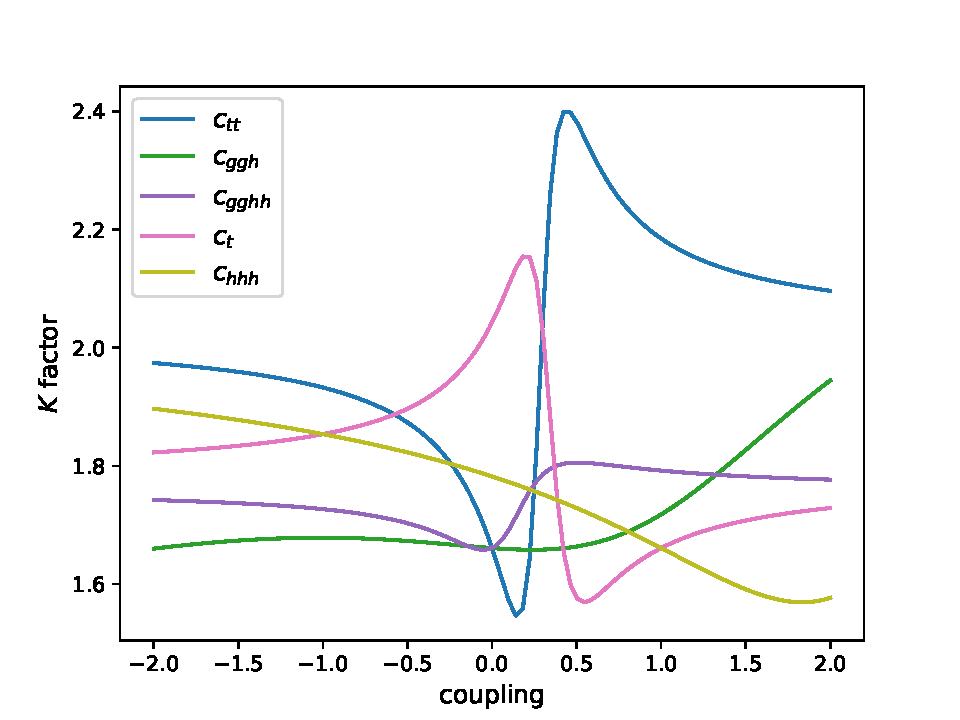
\includegraphics[width=9cm]{\main/section3/plots/Kplot.pdf}
\end{center}
\caption{K-factors for the total cross section at $\sqrt{s}=14$\,TeV as a function of the
  different couplings.}
\label{fig:project_ctt}
\end{figure}
%
In Fig.~\ref{fig:project_ctt} we show the K-factors as a function of
the coupling parameters, with the others fixed to their SM values. 
It shows that the K-factors exhibit a much stronger dependence on the
coupling parameters once the full top quark mass dependence is taken into account when compared to 
the results in the $m_t\to\infty$ limit~\cite{Grober:2015cwa,deFlorian:2017qfk}.
%

Fig.~\ref{fig:ctt_3D} shows the Higgs boson pair invariant mass
distributions as a function of (a) $\ctt$ and (b) $\cgg$ as 3-dimensional heat maps.
In case (a) the other couplings are fixed to their SM values.
We can see that large values of $|\ctt|$ lead to a substantial increase of the cross section, in particular at low $\mhh$ values.
%  
\begin{figure}[ht]
\begin{center}
  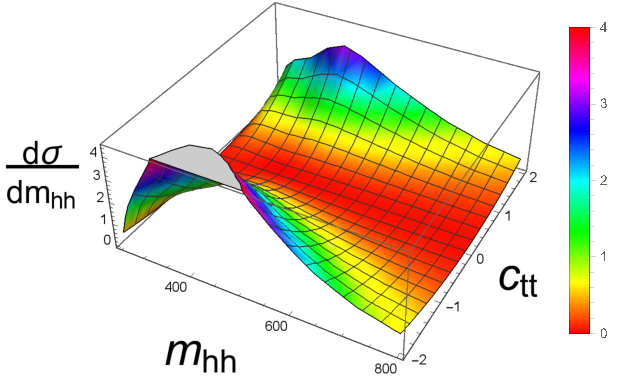
\includegraphics[width=0.45\textwidth]{\main/section3/plots/3D_mhh_ctt.pdf}    
~
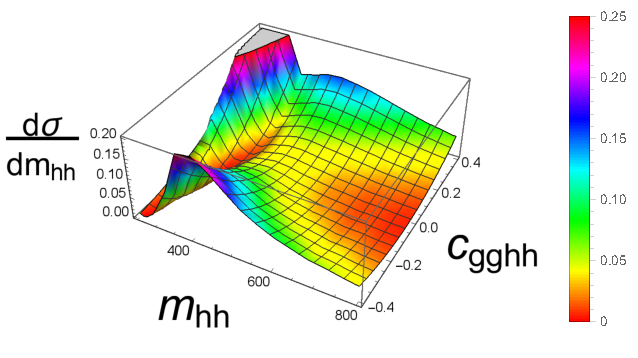
\includegraphics[width=0.5\textwidth]{\main/section3/plots/3D_mhh_cgghh_lam24.pdf}
\end{center}
\caption{3-dimensional visualisation of the $\mhh$ distribution (in units of fb/GeV) at 14\,TeV as a function of (a) $\ctt$  and (b) $\cgg$.  In case (a) all
other couplings are fixed to their SM values, in case (b) $\chhh= 2.4$.}
\label{fig:ctt_3D}
\end{figure}
In case (b) the other couplings are fixed to their SM values except for $\chhh$, which is fixed to $\chhh=2.4$
in order to demonstrate the following point: varying only $\chhh$, the $\mhh$ distribution shows a dip in the differential cross section just below $\mhh\sim 2m_t$ for $\chhh\sim 2.4$, while the low $\mhh$ region gets enhanced for larger values of $\chhh$, see Section~\ref{subsec:varylambda}.
 However, this pattern can get destroyed by non-zero
 Higgs-gluon contact interactions. While $\cg$ is increasingly well constrained meanwhile,
 $\cgg$ still could be relatively large. We can see from Fig.~\ref{fig:ctt_3D}(b) that the dip is not present for very low (negative) $\cgg$ values and also gets very shallow for values of $\cgg\sim 0.4$.
 Therefore it would be premature to conclude that a dip in the $\mhh$ distribution points to a value of $\chhh$ close to 2.4.

We also point out that the LO and NLO $A_i$ coefficients for both the total cross
section and the $\mhh$ distributions at both 14\,TeV and 27\,TeV are
available as ancillary files coming with Ref.~\cite{Buchalla:2018yce}. These data files allow to reconstruct the full NLO result for any point in the 5-dimensional parameter space.


%\clearpage

%\subsubsubsection{Conclusions}
